\documentclass[tikz]{standalone}
\usepackage{tikz,amsmath}
\usetikzlibrary{positioning}
\begin{document}
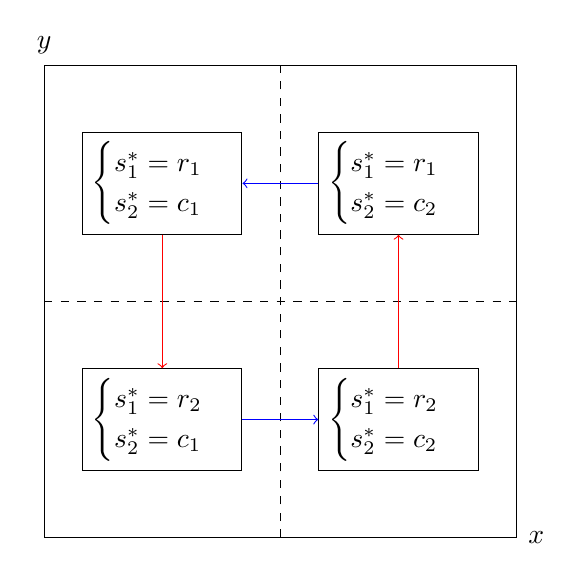
\begin{tikzpicture}
    \draw (-1,-1) rectangle (5,5);
    \draw [dashed] (-1,2) -- (5,2);
    \draw [dashed] (2,-1) -- (2,5);
    \node (11) [rectangle,draw] at (.5,.5) {$\begin{cases}s^*_1=r_2\\s^*_2=c_1\end{cases}$};
    \node (12) [rectangle,draw] at (.5,3.5) {$\begin{cases}s^*_1=r_1\\s^*_2=c_1\end{cases}$};
    \node (21) [rectangle,draw] at (3.5,.5) {$\begin{cases}s^*_1=r_2\\s^*_2=c_2\end{cases}$};
    \node (22) [rectangle,draw] at (3.5,3.5) {$\begin{cases}s^*_1=r_1\\s^*_2=c_2\end{cases}$};
    \draw [->,color=red] (12) -- (11);
    \draw [->,color=red] (21) -- (22);
    \draw [->,color=blue] (11) -- (21);
    \draw [->,color=blue] (22) -- (12);
    \node at (5.25,-1) {$x$};
    \node at (-1, 5.25) {$y$};
\end{tikzpicture}
\end{document}
